% ============================================================
%  SESSION 7 — Next.js Gerçek Kullanım
%  XeLaTeX ile derleyin: xelatex session-07.tex
% ============================================================
\documentclass[12pt, a4paper]{article}

% ---------- Font & Dil ----------
\usepackage{fontspec}
\usepackage[turkish, shorthands=off]{babel}
\setmainfont{Georgia}
\setsansfont{Arial}
\setmonofont{Courier New}

% ---------- Sayfa Düzeni ----------
\usepackage[top=2.2cm, bottom=2.2cm, left=2.4cm, right=2.4cm]{geometry}
\usepackage{parskip}
\setlength{\parindent}{0pt}

% ---------- Renkler ----------
\usepackage{xcolor}
\definecolor{primary}{HTML}{2563EB}
\definecolor{secondary}{HTML}{7C3AED}
\definecolor{accent}{HTML}{059669}
\definecolor{warning}{HTML}{D97706}
\definecolor{danger}{HTML}{DC2626}
\definecolor{lightbg}{HTML}{F1F5F9}
\definecolor{codebg}{HTML}{1E293B}
\definecolor{codefg}{HTML}{E2E8F0}
\definecolor{reactblue}{HTML}{61DAFB}
\definecolor{jsxcol}{HTML}{93C5FD}
\definecolor{propscol}{HTML}{FCA5A5}
\definecolor{statecol}{HTML}{86EFAC}
\definecolor{jskw}{HTML}{93C5FD}
\definecolor{jsstr}{HTML}{86EFAC}
\definecolor{jscomment}{HTML}{94A3B8}
\definecolor{servercol}{HTML}{8B5CF6}
\definecolor{clientcol}{HTML}{F59E0B}
\definecolor{authcol}{HTML}{EC4899}
\definecolor{errorcol}{HTML}{DC2626}

% ---------- Kutular (tcolorbox) ----------
\usepackage[skins, breakable, listings]{tcolorbox}
\tcbuselibrary{skins, breakable, listings}

\newtcolorbox{infobox}[1][]{
  enhanced, breakable,
  colback=primary!8, colframe=primary,
  fonttitle=\bfseries\sffamily,
  title={#1},
  left=6pt, right=6pt, top=4pt, bottom=4pt,
  arc=4pt
}

\newtcolorbox{warningbox}[1][]{
  enhanced, breakable,
  colback=warning!10, colframe=warning,
  fonttitle=\bfseries\sffamily,
  title={#1},
  left=6pt, right=6pt, top=4pt, bottom=4pt,
  arc=4pt
}

\newtcolorbox{practicebox}[1][]{
  enhanced, breakable,
  colback=accent!8, colframe=accent,
  fonttitle=\bfseries\sffamily,
  title={#1},
  left=6pt, right=6pt, top=4pt, bottom=4pt,
  arc=4pt
}

\newtcolorbox{definebox}[1][]{
  enhanced, breakable,
  colback=secondary!7, colframe=secondary,
  fonttitle=\bfseries\sffamily,
  title={#1},
  left=6pt, right=6pt, top=4pt, bottom=4pt,
  arc=4pt
}

\newtcolorbox{dangerbox}[1][]{
  enhanced, breakable,
  colback=danger!7, colframe=danger,
  fonttitle=\bfseries\sffamily,
  title={#1},
  left=6pt, right=6pt, top=4pt, bottom=4pt,
  arc=4pt
}

% ---------- Kod Listeleme ----------
\usepackage{listings}

\lstset{literate=
  {ı}{{\texttt{i}}}1  {İ}{{\texttt{I}}}1
  {ğ}{{\texttt{g}}}1  {Ğ}{{\texttt{G}}}1
  {ş}{{\texttt{s}}}1  {Ş}{{\texttt{S}}}1
  {ü}{{\texttt{u}}}1  {Ü}{{\texttt{U}}}1
  {ö}{{\texttt{o}}}1  {Ö}{{\texttt{O}}}1
  {ç}{{\texttt{c}}}1  {Ç}{{\texttt{C}}}1
}

\lstdefinestyle{jsxstyle}{
  backgroundcolor=\color{codebg},
  basicstyle=\ttfamily\small\color{codefg},
  keywordstyle=\color{jskw}\bfseries,
  stringstyle=\color{jsstr},
  commentstyle=\color{jscomment}\itshape,
  morekeywords={let, const, var, async, await, of, from, import, export,
    default, class, extends, new, return, true, false, null, undefined,
    function, arrow, Promise, fetch, then, catch, finally, try, throw,
    map, filter, reduce, forEach, find, findIndex, some, every,
    console, log, JSON, stringify, parse,
    React, useState, useEffect, useRef, useCallback, useMemo,
    props, children,
    onClick, onChange, onSubmit, onBlur, key, className, style, value,
    disabled, required, placeholder, type, htmlFor, checked,
    div, span, button, input, form, label, h1, h2, h3, p, ul, li, img,
    select, option, textarea, nav, a, main, header, footer,
    interface, type, Link, useRouter, usePathname, useParams,
    Metadata, Layout, Page, params, searchParams,
    cookies, headers, redirect, notFound, NextResponse, NextRequest,
    middleware, matcher, reset, error, useFormStatus},
  morestring=[b]",
  morestring=[b]',
  morestring=[b]`,
  morecomment=[l]{//},
  morecomment=[s]{/*}{*/},
  showstringspaces=false,
  breaklines=true,
  frame=none,
  xleftmargin=8pt, xrightmargin=8pt,
}

\lstdefinestyle{shellstyle}{
  backgroundcolor=\color{codebg},
  basicstyle=\ttfamily\small\color{codefg},
  showstringspaces=false,
  breaklines=true,
  frame=none,
  xleftmargin=8pt, xrightmargin=8pt,
}

% ---------- Grafikler ----------
\usepackage{graphicx}
\usepackage{caption}
\usepackage{tikz}
\usetikzlibrary{arrows.meta, shapes.geometric, positioning, calc}

% ---------- Tablo ----------
\usepackage{booktabs}
\usepackage{tabularx}
\usepackage{array}

% ---------- Başlık Stilleri ----------
\makeatletter
\renewcommand{\section}{%
  \@startsection{section}{1}{\z@}%
    {-1.5ex plus -1ex minus -0.5ex}%
    {0.8ex plus 0.3ex}%
    {\normalfont\Large\bfseries\sffamily\color{primary}}%
}
\renewcommand{\subsection}{%
  \@startsection{subsection}{2}{\z@}%
    {-1.2ex plus -0.8ex minus -0.4ex}%
    {0.5ex plus 0.2ex}%
    {\normalfont\large\bfseries\sffamily\color{secondary}}%
}
\renewcommand{\subsubsection}{%
  \@startsection{subsubsection}{3}{\z@}%
    {-1ex plus -0.6ex minus -0.3ex}%
    {0.4ex}%
    {\normalfont\normalsize\bfseries\sffamily\color{accent}}%
}
\makeatother

% ---------- Üstbilgi / Altbilgi ----------
\usepackage{fancyhdr}
\setlength{\headheight}{14pt}
\pagestyle{fancy}
\fancyhf{}
\fancyhead[L]{\small\sffamily\color{gray} Front-end + Next.js Eğitimi}
\fancyhead[R]{\small\sffamily\color{gray} Session 7 --- Next.js Gerçek Kullanım}
\fancyfoot[C]{\small\sffamily\color{gray} \thepage}
\renewcommand{\headrulewidth}{0.4pt}

% ---------- Diğer ----------
\usepackage{enumitem}
\setlist[itemize]{leftmargin=1.5em, itemsep=2pt}
\setlist[enumerate]{leftmargin=1.5em, itemsep=2pt}
\usepackage{hyperref}
\hypersetup{colorlinks=true, linkcolor=primary, urlcolor=primary}
\usepackage{fontawesome5}

% ---------- Yardımcı Komut ----------
\newcommand{\timebadge}[1]{%
  \noindent
  \colorbox{primary}{\color{white}\sffamily\bfseries\small\strut~~\faStopwatch~~#1~~}%
  \par\vspace{4pt}%
}

\newcommand{\jsinline}[1]{\texttt{\color{primary}#1}}

% ============================================================
\begin{document}

% ============================================================
%  KAPAK
% ============================================================
\thispagestyle{empty}

\begin{tikzpicture}[remember picture, overlay]
  \fill[primary] (current page.north west)
    rectangle ++(\paperwidth, -8.0cm);
  \fill[secondary] (current page.north west) ++(0,-7.8cm)
    rectangle ++(\paperwidth, -0.28cm);
\end{tikzpicture}

\vspace*{1.6cm}
{\color{white}\sffamily
  \hspace{1.2cm}{\small SESSION 7 / 8 \quad|\quad 13 Mayıs 2026 \quad|\quad~90 dakika}\\[12pt]
  \hspace{1.2cm}{\fontsize{30}{36}\selectfont\bfseries Next.js Gerçek Kullanım}\\[8pt]
  \hspace{1.2cm}{\Large API, Error Handling, Auth Flow}
}

\vspace{0.9cm}

\vspace{0.1cm}

\begin{tcolorbox}[enhanced,
  colback=lightbg, colframe=gray!30, arc=4pt,
  title={\sffamily\bfseries\color{primary}\faStream\quad Session Akışı},
  fonttitle=\bfseries\sffamily]
\sffamily\small
\begin{tabularx}{\textwidth}{>{\bfseries\color{primary}}l X l}
\toprule
Süre & Konu & Anahtar Kavramlar \\
\midrule
0--25 dk  & API Entegrasyonu \& Loading       & Server vs Client, "use client", Suspense \\
25--50 dk & Error Handling \& UI Feedback     & error.tsx, try/catch, toast \\
50--70 dk & Auth Flow \& Protected Route       & cookie, middleware, session \\
70--90 dk & \textcolor{accent}{Pratik: Login + Protected} & form action, cookie, redirect \\
\bottomrule
\end{tabularx}
\end{tcolorbox}

% ============================================================
\clearpage
\section{\faExchange*\ API Entegrasyonu ve Loading State}
\timebadge{0--25 dakika}

\subsection{Server Component vs Client Component}

Session 6'da Next.js'in varsayılan olarak \textbf{server component} kullandığını
gördük. Ama gerçek projelerde \texttt{useState}, \texttt{onClick} gibi
interaktif şeylere ihtiyacımız var. Bunlar sadece \textbf{client component}'lerde
çalışır.

\vspace{6pt}

\begin{center}
\begin{tikzpicture}[
  box/.style={draw=#1, fill=#1!10, rounded corners=5pt,
    minimum width=6.0cm, minimum height=3.0cm,
    font=\sffamily\small, text=#1!50!black, align=left,
    text width=5.4cm}
]
  \node[box=servercol] (server) at (-3.6, 0)
    {\textbf{\color{servercol}Server Component (varsayılan)}\\[2pt]
     \faCheck~ async/await ile veri çekme\\
     \faCheck~ DB / API key güvenli\\
     \faCheck~ JS bundle'a eklenmez\\
     \faTimes~ useState, useEffect yok\\
     \faTimes~ onClick, onChange yok\\
     \faTimes~ Browser API'leri yok};

  \node[box=clientcol] (client) at (3.6, 0)
    {\textbf{\color{clientcol}Client Component ("use client")}\\[2pt]
     \faCheck~ useState, useEffect var\\
     \faCheck~ Event handler'lar var\\
     \faCheck~ Browser API'leri\\
     \faTimes~ JS bundle'a eklenir\\
     \faTimes~ Doğrudan DB erişimi yok\\
     \faTimes~ Async olamaz};
\end{tikzpicture}
\end{center}

\vspace{6pt}

\begin{definebox}["use client" Directive]
Bir dosyanın \textbf{en üstüne} \texttt{"use client";} yazarsanız o dosya
ve içinden import ettikleri \textbf{client component} olur.
\texttt{useState}, \texttt{onClick}, \texttt{useEffect} kullanabilirsiniz.
\end{definebox}

\vspace{6pt}

\begin{tcolorbox}[enhanced, colback=codebg, colframe=gray!30,
    colbacktitle=clientcol!85!black, coltitle=white, arc=4pt,
    title={\sffamily\bfseries\small Client Component Örneği}]
\begin{lstlisting}[style=jsxstyle]
"use client"; // <-- En ust satir

import { useState } from "react";

export default function Counter() {
  const [count, setCount] = useState(0);

  return (
    <div>
      <p>Count: {count}</p>
      <button onClick={() => setCount(count + 1)}>
        Artir
      </button>
    </div>
  );
}
\end{lstlisting}
\end{tcolorbox}

% ----------------------------------------------------------
\newpage
\subsection{Hangi Component'i Ne Zaman Seçmeli?}

\begin{tcolorbox}[enhanced, colback=lightbg, colframe=gray!30, arc=4pt]
\sffamily\small
\begin{tabularx}{\textwidth}{>{\bfseries\color{primary}}l X}
\toprule
Senaryo & Hangisi? \\
\midrule
Sayfa içeriği veri çekiyor (statik gösterim)     & Server \\
Buton, input, form gibi etkileşim var            & Client \\
Search bar, filtre, modal                        & Client \\
SEO için önemli statik içerik                    & Server \\
localStorage, window kullanılıyor                & Client \\
API key kullanılıyor                             & Server (zorunlu!) \\
\bottomrule
\end{tabularx}
\end{tcolorbox}

\vspace{6pt}

\begin{infobox}[\faLightbulb\ Karma Yaklaşım --- En Yaygın]
Sayfanın \textbf{kabuğu server component}, \textbf{etkileşimli kısımları}
küçük client component'lere ayrılır. Bu sayede JS bundle minimum,
performans maksimum olur.

\vspace{4pt}
\textbf{Server component'ler, içinde client component'leri render edebilir.}
Tersi mümkün değildir (client içinden server import edilemez).
\end{infobox}

\vspace{6pt}

\subsubsection{Karma Yaklaşım Örneği}

\begin{tcolorbox}[enhanced, colback=codebg, colframe=gray!30,
    colbacktitle=primary!85!black, coltitle=white, arc=4pt,
    title={\sffamily\bfseries\small src/app/products/page.tsx (Server)}]
\begin{lstlisting}[style=jsxstyle]
import AddToCartButton from "./AddToCartButton";

interface Product {
  id: number;
  title: string;
  price: number;
}

export default async function ProductsPage() {
  const res = await fetch("https://fakestoreapi.com/products");
  const products: Product[] = await res.json();

  return (
    <div>
      <h1>Urunler</h1>
      {products.map(p => (
        <div key={p.id}>
          <h2>{p.title}</h2>
          <p>{p.price} TL</p>
          <AddToCartButton productId={p.id} />
        </div>
      ))}
    </div>
  );
}
\end{lstlisting}
\end{tcolorbox}

\vspace{4pt}

\begin{tcolorbox}[enhanced, colback=codebg, colframe=gray!30,
    colbacktitle=clientcol!85!black, coltitle=white, arc=4pt,
    title={\sffamily\bfseries\small src/app/products/AddToCartButton.tsx (Client)}]
\begin{lstlisting}[style=jsxstyle]
"use client";

import { useState } from "react";

export default function AddToCartButton({ productId }: { productId: number }) {
  const [added, setAdded] = useState(false);

  return (
    <button onClick={() => setAdded(true)}>
      {added ? "Eklendi" : "Sepete Ekle"}
    </button>
  );
}
\end{lstlisting}
\end{tcolorbox}

% ----------------------------------------------------------
\newpage
\subsection{Loading State Yönetimi}

\subsubsection{Server Component'te --- loading.tsx}

Server component'te veri \texttt{await} ile çekiliyor ve sayfa
hazır olunca render ediliyor. Bu sırada \texttt{loading.tsx}
otomatik gösterilir.

\vspace{6pt}

\begin{center}
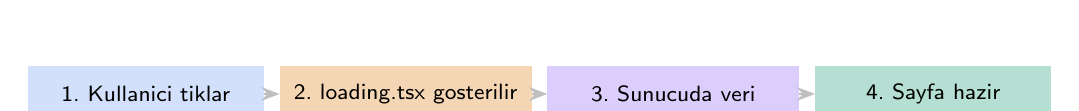
\begin{tikzpicture}[node distance=0.4cm, >=Stealth, font=\sffamily\footnotesize]
  \fill[primary!20] (0.0, 0.5) rectangle (3.0, 1.2);
  \node at (1.5, 0.85) {1. Kullanici tiklar};
  \draw[->, thick, gray!50] (3.0, 0.85) -- (3.2, 0.85);

  \fill[warning!30] (3.2, 0.5) rectangle (6.4, 1.2);
  \node at (4.8, 0.85) {2. loading.tsx gosterilir};
  \draw[->, thick, gray!50] (6.4, 0.85) -- (6.6, 0.85);

  \fill[servercol!30] (6.6, 0.5) rectangle (9.8, 1.2);
  \node at (8.2, 0.85) {3. Sunucuda veri};
  \draw[->, thick, gray!50] (9.8, 0.85) -- (10.0, 0.85);

  \fill[accent!30] (10.0, 0.5) rectangle (13.0, 1.2);
  \node at (11.5, 0.85) {4. Sayfa hazir};
\end{tikzpicture}
\end{center}

\vspace{6pt}

\begin{tcolorbox}[enhanced, colback=codebg, colframe=gray!30,
    colbacktitle=warning!85!black, coltitle=white, arc=4pt,
    title={\sffamily\bfseries\small src/app/products/loading.tsx}]
\begin{lstlisting}[style=jsxstyle]
// Sayfanin verisi yuklenirken otomatik gosterilir
export default function Loading() {
  return (
    <div style={{ padding: 40 }}>
      <p>Urunler yukleniyor...</p>
      {/* Skeleton UI da konabilir --- icerik genisliginde gri kutular */}
    </div>
  );
}
\end{lstlisting}
\end{tcolorbox}

\vspace{6pt}

\subsubsection{Client Component'te --- Manual Loading State}

Client tarafında veri çekiyorsak loading'i kendimiz yönetiriz:

\begin{tcolorbox}[enhanced, colback=codebg, colframe=gray!30,
    colbacktitle=clientcol!85!black, coltitle=white, arc=4pt,
    title={\sffamily\bfseries\small Client'ta Loading}]
\begin{lstlisting}[style=jsxstyle]
"use client";

import { useState, useEffect } from "react";

export default function UserList() {
  const [users, setUsers] = useState<User[]>([]);
  const [loading, setLoading] = useState(true);

  useEffect(() => {
    fetch("/api/users")
      .then(r => r.json())
      .then(data => {
        setUsers(data);
        setLoading(false);
      });
  }, []);

  if (loading) return <p>Yukleniyor...</p>;

  return <ul>{users.map(u => <li key={u.id}>{u.name}</li>)}</ul>;
}
\end{lstlisting}
\end{tcolorbox}

\vspace{6pt}

\begin{infobox}[\faLightbulb\ Hangi Yöntemi Seçmeli?]
\begin{itemize}
  \item Sayfa açılırken \textbf{veri zaten gerekiyorsa} $\rightarrow$ Server component + \texttt{loading.tsx}
  \item Veri \textbf{kullanıcı etkileşimi} ile gelecekse $\rightarrow$ Client component + manuel state
  \item Veri \textbf{filtreleme} / arama ile geliyorsa $\rightarrow$ Client component
\end{itemize}
\end{infobox}

% ============================================================
\newpage
\section{\faExclamationTriangle\ Error Handling ve UI Feedback}
\timebadge{25--50 dakika}

\subsection{Hataların Yaşam Döngüsü}

API çağrıları her zaman başarılı olmaz. Network kopabilir, sunucu 500
dönebilir, bulunamayan kaynak için 404 gelebilir. Bunları \textbf{yakalayıp}
kullanıcıya anlamlı bir mesaj göstermeliyiz.

\vspace{6pt}

\begin{center}
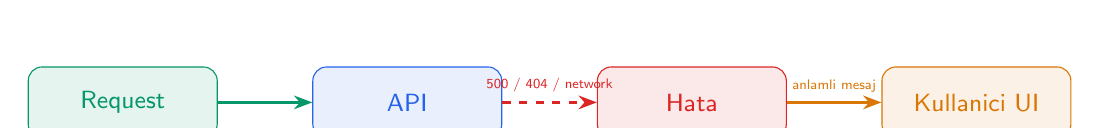
\begin{tikzpicture}[>=Stealth, font=\sffamily\small]
  \node[draw=accent, fill=accent!10, rounded corners=5pt,
        minimum width=2.4cm, minimum height=0.9cm, text=accent]
        (req) at (0,0) {Request};

  \node[draw=primary, fill=primary!10, rounded corners=5pt,
        minimum width=2.4cm, minimum height=0.9cm, text=primary,
        right=1.2cm of req] (api) {API};

  \node[draw=danger, fill=danger!10, rounded corners=5pt,
        minimum width=2.4cm, minimum height=0.9cm, text=danger,
        right=1.2cm of api] (err) {Hata};

  \node[draw=warning, fill=warning!10, rounded corners=5pt,
        minimum width=2.4cm, minimum height=0.9cm, text=warning,
        right=1.2cm of err] (ui) {Kullanici UI};

  \draw[->, thick, accent] (req) -- (api);
  \draw[->, thick, danger, dashed] (api) -- node[above, font=\sffamily\tiny]{500 / 404 / network} (err);
  \draw[->, thick, warning] (err) -- node[above, font=\sffamily\tiny]{anlamli mesaj} (ui);
\end{tikzpicture}
\end{center}

\vspace{6pt}

\begin{warningbox}[\faExclamationTriangle\ Yapılmaması Gerekenler]
\begin{itemize}
  \item Sessizce \texttt{console.log(err)} ile bırakmak --- kullanıcı bir şey olduğunu bilmez
  \item Ham hata mesajını göstermek --- \texttt{TypeError: undefined is not a function} kullanıcıya bir şey anlatmaz
  \item Tüm sayfa için tek bir ``Bir hata oluştu'' --- nedeni bilinmez
  \item Beyaz ekran --- ``site mi çöktü?'' sorusu doğar
\end{itemize}
\end{warningbox}

% ----------------------------------------------------------
\subsection{Server Component'te Hata Yakalama}

\subsubsection{Yöntem 1 --- try / catch}

\begin{tcolorbox}[enhanced, colback=codebg, colframe=gray!30,
    colbacktitle=servercol!85!black, coltitle=white, arc=4pt,
    title={\sffamily\bfseries\small try / catch ile Hata Yönetimi}]
\begin{lstlisting}[style=jsxstyle]
export default async function ProductsPage() {
  try {
    const res = await fetch("https://api.example.com/products");

    if (!res.ok) {
      throw new Error(`HTTP ${res.status}: ${res.statusText}`);
    }

    const products = await res.json();

    return (
      <ul>
        {products.map(p => <li key={p.id}>{p.title}</li>)}
      </ul>
    );
  } catch (err) {
    return (
      <div style={{ padding: 24, color: "#dc2626" }}>
        <h2>Urunler yuklenemedi</h2>
        <p>Lutfen daha sonra tekrar deneyin.</p>
      </div>
    );
  }
}
\end{lstlisting}
\end{tcolorbox}

\vspace{6pt}

\subsubsection{Yöntem 2 --- notFound() ile 404'e Yönlendirme}

\begin{tcolorbox}[enhanced, colback=codebg, colframe=gray!30,
    colbacktitle=servercol!85!black, coltitle=white, arc=4pt,
    title={\sffamily\bfseries\small Bulunamayan Kaynak için notFound()}]
\begin{lstlisting}[style=jsxstyle]
import { notFound } from "next/navigation";

export default async function ProductDetailPage({ params }) {
  const { id } = await params;

  const res = await fetch(`https://api.example.com/products/${id}`);

  if (res.status === 404) {
    notFound(); // -> not-found.tsx gosterilir
  }

  if (!res.ok) {
    throw new Error("API hatasi"); // -> error.tsx gosterilir
  }

  const product = await res.json();
  return <h1>{product.title}</h1>;
}
\end{lstlisting}
\end{tcolorbox}

% ----------------------------------------------------------
\newpage
\subsection{error.tsx --- Otomatik Error Boundary}

\begin{definebox}[error.tsx Nedir?]
Next.js'in özel dosyalarından biri. Bir sayfada veya layout'unda
\textbf{yakalanmamış hata} oluşursa, en yakın \texttt{error.tsx}
otomatik gösterilir. React'taki Error Boundary'nin Next.js
versiyonudur.
\end{definebox}

\vspace{6pt}

\begin{tcolorbox}[enhanced, colback=codebg, colframe=gray!30,
    colbacktitle=errorcol!85!black, coltitle=white, arc=4pt,
    title={\sffamily\bfseries\small src/app/products/error.tsx}]
\begin{lstlisting}[style=jsxstyle]
"use client"; // error.tsx HER ZAMAN client component olmali

interface Props {
  error: Error & { digest?: string };
  reset: () => void;
}

export default function Error({ error, reset }: Props) {
  return (
    <div style={{ padding: 40, textAlign: "center" }}>
      <h2>Bir seyler ters gitti</h2>
      <p style={{ color: "#64748b" }}>{error.message}</p>
      <button
        onClick={reset}
        style={{
          padding: "10px 20px",
          background: "#2563eb",
          color: "white",
          border: "none",
          borderRadius: 8,
          cursor: "pointer",
        }}
      >
        Tekrar Dene
      </button>
    </div>
  );
}
\end{lstlisting}
\end{tcolorbox}

\vspace{6pt}

\begin{tcolorbox}[enhanced, colback=lightbg, colframe=gray!30, arc=4pt]
\sffamily\small
\begin{tabularx}{\textwidth}{>{\ttfamily\color{primary}}l X}
\toprule
\normalfont\bfseries Prop & \normalfont\bfseries Açıklama \\
\midrule
error          & Yakalanan hata objesi (\texttt{message}, \texttt{digest}\ldots) \\
reset          & Çağrılınca segment yeniden render edilir --- ``Tekrar Dene'' butonu için \\
\bottomrule
\end{tabularx}
\end{tcolorbox}

\vspace{6pt}

\begin{infobox}[\faSitemap\ Error Hiyerarşisi]
Bir sayfada hata olduğunda Next.js \textbf{en yakın} \texttt{error.tsx}'i arar:
\vspace{4pt}
\texttt{products/[id]/error.tsx} $\rightarrow$
\texttt{products/error.tsx} $\rightarrow$
\texttt{global-error.tsx}

\vspace{4pt}
Her segment kendi error.tsx'ini tanımlayarak farklı UI gösterebilir.
\end{infobox}

% ----------------------------------------------------------
\newpage
\subsection{Client Component'te Hata Yönetimi}

Client tarafında veri çekiyorsak, hatayı \textbf{state}'te tutarız.
Session 4'te öğrendiğimiz \textbf{Loading / Error / Data} kalıbı:

\vspace{6pt}

\begin{tcolorbox}[enhanced, colback=codebg, colframe=gray!30,
    colbacktitle=clientcol!85!black, coltitle=white, arc=4pt,
    title={\sffamily\bfseries\small Client'ta Loading + Error + Data}]
\begin{lstlisting}[style=jsxstyle]
"use client";

import { useState, useEffect } from "react";

export default function UserList() {
  const [data, setData] = useState<User[] | null>(null);
  const [loading, setLoading] = useState(true);
  const [error, setError] = useState<string | null>(null);

  useEffect(() => {
    async function load() {
      try {
        const res = await fetch("/api/users");
        if (!res.ok) throw new Error(`HTTP ${res.status}`);
        const json = await res.json();
        setData(json);
      } catch (err) {
        setError(err instanceof Error ? err.message : "Bilinmeyen hata");
      } finally {
        setLoading(false);
      }
    }
    load();
  }, []);

  if (loading) return <p>Yukleniyor...</p>;
  if (error)   return <p style={{ color: "red" }}>Hata: {error}</p>;
  if (!data)   return <p>Veri bulunamadi.</p>;

  return <ul>{data.map(u => <li key={u.id}>{u.name}</li>)}</ul>;
}
\end{lstlisting}
\end{tcolorbox}

\vspace{6pt}

\subsection{UI Feedback Pattern'leri}

\begin{tcolorbox}[enhanced, colback=lightbg, colframe=gray!30, arc=4pt]
\sffamily\small
\begin{tabularx}{\textwidth}{>{\bfseries\color{primary}}l X}
\toprule
Pattern & Ne Zaman Kullanılır? \\
\midrule
Inline mesaj &
  Form input altında hata mesajı (Session 4'te gördük) \\[4pt]
Toast / Snackbar &
  Geçici bildirim --- ``Kaydedildi'', ``Silindi'' (3-5 sn görünür) \\[4pt]
Loading spinner &
  Buton üzerinde işlem sırasında (\texttt{disabled} + animasyon) \\[4pt]
Empty state &
  Liste boşsa \textbf{anlamlı mesaj} --- ``Henüz görev yok, ilk ekleyen siz olun!'' \\[4pt]
Error page &
  Tüm sayfa çöktüyse error.tsx ile genel hata sayfası \\[4pt]
Optimistic UI &
  İşlem bitmeden UI'ı önden güncelle, hata olursa geri al \\
\bottomrule
\end{tabularx}
\end{tcolorbox}

\vspace{6pt}

\begin{warningbox}[\faLightbulb\ Kullanıcı Dostu Mesaj Yazma]
\begin{itemize}
  \item ``Bir hata oluştu'' yerine: ``Ürünler şu an yüklenemiyor, birazdan tekrar deneyin.''
  \item ``500 Internal Server Error'' yerine: ``Sunucumuzda geçici bir sorun var.''
  \item Mümkünse \textbf{ne yapacağını söyleyin}: ``Tekrar dene'' butonu, ``destek ekibine yazın'' linki vs.
\end{itemize}
\end{warningbox}

% ============================================================
\newpage
\section{\faLock\ Auth Flow ve Protected Route}
\timebadge{50--70 dakika}

\subsection{Authentication Nedir?}

\begin{definebox}[Auth Temelleri]
\textbf{Authentication (kimlik doğrulama):} ``Kim olduğunu kanıtla''
(login, email + şifre).\\
\textbf{Authorization (yetkilendirme):} ``Bu işlemi yapmaya yetkin var mı?''
(admin sayfasını görebilir mi?).
\end{definebox}

\vspace{6pt}

\subsubsection{Tipik Login Akışı}

\begin{center}
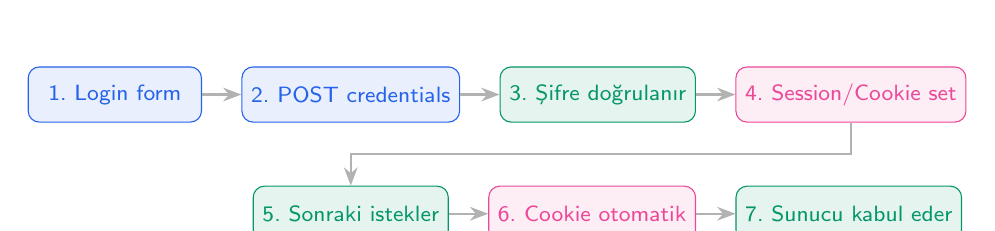
\begin{tikzpicture}[>=Stealth, font=\sffamily\footnotesize, node distance=0.6cm]

  \node[draw=primary, fill=primary!10, rounded corners=4pt,
        minimum width=2.2cm, minimum height=0.7cm, text=primary]
        (login) at (0,0) {1. Login form};

  \node[draw=primary, fill=primary!10, rounded corners=4pt,
        minimum width=2.4cm, minimum height=0.7cm, text=primary,
        right=0.5cm of login] (post) {2. POST credentials};

  \node[draw=accent, fill=accent!10, rounded corners=4pt,
        minimum width=2.4cm, minimum height=0.7cm, text=accent,
        right=0.5cm of post] (verify) {3. Şifre doğrulanır};

  \node[draw=authcol, fill=authcol!10, rounded corners=4pt,
        minimum width=2.6cm, minimum height=0.7cm, text=authcol,
        right=0.5cm of verify] (cookie) {4. Session/Cookie set};

  \node[draw=accent, fill=accent!10, rounded corners=4pt,
        minimum width=2.4cm, minimum height=0.7cm, text=accent,
        below=0.8cm of post] (next) {5. Sonraki istekler};

  \node[draw=authcol, fill=authcol!10, rounded corners=4pt,
        minimum width=2.4cm, minimum height=0.7cm, text=authcol,
        right=0.5cm of next] (auto) {6. Cookie otomatik};

  \node[draw=accent, fill=accent!10, rounded corners=4pt,
        minimum width=2.6cm, minimum height=0.7cm, text=accent,
        right=0.5cm of auto] (allow) {7. Sunucu kabul eder};

  \draw[->, thick, gray!60] (login) -- (post);
  \draw[->, thick, gray!60] (post) -- (verify);
  \draw[->, thick, gray!60] (verify) -- (cookie);
  \draw[->, thick, gray!60] (cookie.south) -- ++(0,-0.4) -| (next.north);
  \draw[->, thick, gray!60] (next) -- (auto);
  \draw[->, thick, gray!60] (auto) -- (allow);
\end{tikzpicture}
\end{center}

\vspace{6pt}

\begin{tcolorbox}[enhanced, colback=lightbg, colframe=gray!30, arc=4pt]
\sffamily\small
\begin{tabularx}{\textwidth}{>{\bfseries\color{primary}}l X}
\toprule
Yöntem & Açıklama \\
\midrule
Cookie (httpOnly) &
  Sunucu set eder, browser otomatik gönderir. \textbf{En güvenli} ---
  JavaScript erişemez, XSS koruması var. \\[4pt]
JWT (localStorage) &
  Token'ı client saklar, header'da gönderir. XSS riski var. \\[4pt]
Session (sunucu) &
  Sunucuda session store; cookie sadece session ID tutar. \\
\bottomrule
\end{tabularx}
\end{tcolorbox}

\vspace{6pt}

\begin{infobox}[\faLightbulb\ Bu Kursta Yaklaşım]
En basit ve güvenli olan \textbf{httpOnly cookie} yaklaşımını kullanacağız.
Gerçek projede arkadaki sistem genelde JWT veya session olsa da,
\textbf{Next.js tarafından bakınca tek mesele cookie'nin var olup olmadığıdır}.
\end{infobox}

% ----------------------------------------------------------
\newpage
\subsection{Next.js'te Cookie Okuma}

Server component'te \texttt{cookies()} fonksiyonu ile cookie'leri okuyabiliriz:

\vspace{6pt}

\begin{tcolorbox}[enhanced, colback=codebg, colframe=gray!30,
    colbacktitle=authcol!85!black, coltitle=white, arc=4pt,
    title={\sffamily\bfseries\small Server Component'te Cookie}]
\begin{lstlisting}[style=jsxstyle]
import { cookies } from "next/headers";

export default async function DashboardPage() {
  const cookieStore = await cookies();
  const session = cookieStore.get("session");

  if (!session) {
    return <p>Lutfen giris yapin.</p>;
  }

  return <h1>Hosgeldin, {session.value}!</h1>;
}
\end{lstlisting}
\end{tcolorbox}

\vspace{6pt}

\subsection{Cookie Set Etme --- Server Action}

Form gönderildiğinde sunucuda kontrol yapıp cookie set etmek için
\textbf{server action} kullanırız:

\vspace{6pt}

\begin{tcolorbox}[enhanced, colback=codebg, colframe=gray!30,
    colbacktitle=authcol!85!black, coltitle=white, arc=4pt,
    title={\sffamily\bfseries\small src/app/login/actions.ts}]
\begin{lstlisting}[style=jsxstyle]
"use server"; // <-- Server action directive

import { cookies } from "next/headers";
import { redirect } from "next/navigation";

export async function login(formData: FormData) {
  const email = formData.get("email") as string;
  const password = formData.get("password") as string;

  // Gercek projede DB'den kontrol edilir
  if (email === "admin@example.com" && password === "123456") {
    const cookieStore = await cookies();
    cookieStore.set("session", email, {
      httpOnly: true,
      secure: true,
      maxAge: 60 * 60 * 24, // 1 gun
      path: "/",
    });
    redirect("/dashboard");
  }

  // Hata durumu: form sayfasina hata mesaji ile geri don
  return { error: "Email veya sifre yanlis" };
}
\end{lstlisting}
\end{tcolorbox}

\vspace{6pt}

\begin{definebox}[Server Action]
\texttt{"use server"} ile işaretlenmiş fonksiyonlar, sunucuda çalışan
fonksiyonlardır. Form'un \texttt{action} prop'una doğrudan verilebilir.
Browser otomatik olarak POST request gönderir, sonuç sayfaya döner.
\end{definebox}

% ----------------------------------------------------------
\subsection{Protected Route --- Layout ile Koruma}

Bir route grubunu korumak için layout'ta \texttt{cookies()} ile kontrol
yapıp gerekirse \texttt{redirect} kullanırız:

\vspace{6pt}

\begin{tcolorbox}[enhanced, colback=codebg, colframe=gray!30,
    colbacktitle=authcol!85!black, coltitle=white, arc=4pt,
    title={\sffamily\bfseries\small src/app/dashboard/layout.tsx}]
\begin{lstlisting}[style=jsxstyle]
import { cookies } from "next/headers";
import { redirect } from "next/navigation";

export default async function DashboardLayout({
  children,
}: {
  children: React.ReactNode;
}) {
  const cookieStore = await cookies();
  const session = cookieStore.get("session");

  if (!session) {
    redirect("/login"); // <-- Cookie yoksa login'e yonlendir
  }

  return (
    <div>
      <header>
        <p>Giris yapan: {session.value}</p>
      </header>
      {children}
    </div>
  );
}
\end{lstlisting}
\end{tcolorbox}

\vspace{6pt}

\begin{infobox}[\faShieldVirus\ Korumalı Layout'un Gücü]
\texttt{dashboard/layout.tsx}'te kontrol yaptığımız için
\textbf{dashboard altındaki tüm sayfalar} otomatik korunur:
\texttt{/dashboard}, \texttt{/dashboard/settings},
\texttt{/dashboard/profile}\ldots Her sayfa için tek tek kontrol
yazmaya gerek yok.
\end{infobox}

% ----------------------------------------------------------
\newpage
\subsection{Middleware --- Daha Gelişmiş Koruma}

\texttt{middleware.ts}, her istek \textbf{sayfaya gelmeden önce} çalışan
bir fonksiyondur. Auth kontrolü için en güçlü yer:

\vspace{6pt}

\begin{tcolorbox}[enhanced, colback=codebg, colframe=gray!30,
    colbacktitle=authcol!85!black, coltitle=white, arc=4pt,
    title={\sffamily\bfseries\small src/middleware.ts (proje köküne yakın)}]
\begin{lstlisting}[style=jsxstyle]
import { NextResponse } from "next/server";
import type { NextRequest } from "next/server";

export function middleware(request: NextRequest) {
  const session = request.cookies.get("session");

  if (!session) {
    // Cookie yoksa login sayfasina yonlendir
    return NextResponse.redirect(new URL("/login", request.url));
  }

  return NextResponse.next(); // Devam et
}

// Hangi route'larda calisacagini belirt
export const config = {
  matcher: ["/dashboard/:path*", "/profile/:path*"],
};
\end{lstlisting}
\end{tcolorbox}

\vspace{6pt}

\begin{tcolorbox}[enhanced, colback=lightbg, colframe=gray!30, arc=4pt]
\sffamily\small
\begin{tabularx}{\textwidth}{>{\bfseries\color{primary}}l X X}
\toprule
& Layout-based & Middleware-based \\
\midrule
Konumu & Her klasörün layout.tsx'i & Tek dosya (\texttt{middleware.ts}) \\[3pt]
Çalışma zamanı & Sayfa render edilirken & İstek geldiğinde, render'dan önce \\[3pt]
Performans & Sayfaya kadar gelir, sonra redirect & Erken redirect, daha hızlı \\[3pt]
Karmaşık logic & Component'lerle birlikte & Sadeleştirilmiş --- Edge runtime \\[3pt]
Önerilen & Basit uygulamalar & Çoklu korumalı route'lar \\
\bottomrule
\end{tabularx}
\end{tcolorbox}

% ============================================================
\newpage
\section{\faHammer\ Pratik: Login + Protected Page}
\timebadge{70--90 dakika}

\begin{practicebox}[\faTasks\ Pratik Hedef]
Basit bir login sistemi ile korumalı sayfa örneği yapalım:
\begin{enumerate}
  \item \texttt{/login} --- Email + şifre formu (client component, hata gösterimi)
  \item Form gönderilince server action ile cookie set
  \item \texttt{/dashboard} --- Korumalı sayfa (cookie yoksa /login'e yönlendirir)
  \item \texttt{/dashboard/profile} --- Aynı korumayı miras alır (nested layout)
  \item Logout butonu --- cookie siler, /login'e yönlendirir
\end{enumerate}
\end{practicebox}

\vspace{8pt}

\subsection{Dosya Yapısı}

\begin{center}
\begin{tikzpicture}[font=\ttfamily\small]
  \node[anchor=west, primary] at (0,    3.0) {src/app/};
  \node[anchor=west, secondary] at (0.5,  2.4) {├── layout.tsx};
  \node[anchor=west, secondary] at (0.5,  1.8) {├── page.tsx};
  \node[anchor=west, primary] at (0.5,  1.2) {├── login/};
  \node[anchor=west, secondary] at (1.0,  0.6) {│   ├── page.tsx};
  \node[anchor=west, secondary] at (1.0,  0.0) {│   ├── actions.ts};
  \node[anchor=west, secondary] at (1.0, -0.6) {│   └── LoginForm.tsx};
  \node[anchor=west, primary] at (0.5, -1.2) {└── dashboard/};
  \node[anchor=west, secondary] at (1.0, -1.8) {\quad├── layout.tsx};
  \node[anchor=west, secondary] at (1.0, -2.4) {\quad├── page.tsx};
  \node[anchor=west, secondary] at (1.0, -3.0) {\quad├── LogoutButton.tsx};
  \node[anchor=west, primary] at (1.0, -3.6) {\quad└── profile/};
  \node[anchor=west, secondary] at (1.5, -4.2) {\quad\quad\quad└── page.tsx};
\end{tikzpicture}
\end{center}

\vspace{8pt}

\subsection{Adım 1 --- Server Action}

\begin{tcolorbox}[enhanced, colback=codebg, colframe=gray!30,
    colbacktitle=authcol!85!black, coltitle=white, arc=4pt,
    title={\sffamily\bfseries\small src/app/login/actions.ts}]
\begin{lstlisting}[style=jsxstyle]
"use server";

import { cookies } from "next/headers";
import { redirect } from "next/navigation";

export async function login(_prevState: unknown, formData: FormData) {
  const email = formData.get("email") as string;
  const password = formData.get("password") as string;

  // Demo amacli sabit kontrol --- gercek projede DB
  if (email !== "admin@example.com" || password !== "123456") {
    return { error: "Email veya sifre yanlis." };
  }

  const cookieStore = await cookies();
  cookieStore.set("session", email, {
    httpOnly: true,
    maxAge: 60 * 60 * 24,
    path: "/",
  });

  redirect("/dashboard");
}

export async function logout() {
  const cookieStore = await cookies();
  cookieStore.delete("session");
  redirect("/login");
}
\end{lstlisting}
\end{tcolorbox}

% ----------------------------------------------------------
\newpage
\subsection{Adım 2 --- Login Formu}

\begin{tcolorbox}[enhanced, colback=codebg, colframe=gray!30,
    colbacktitle=clientcol!85!black, coltitle=white, arc=4pt,
    title={\sffamily\bfseries\small src/app/login/LoginForm.tsx (Client)}]
\begin{lstlisting}[style=jsxstyle]
"use client";

import { useActionState } from "react";
import { login } from "./actions";

export default function LoginForm() {
  const [state, formAction, pending] = useActionState(login, null);

  return (
    <form action={formAction} style={{ maxWidth: 320, margin: "0 auto" }}>
      <h1>Giris Yap</h1>

      <input
        name="email"
        type="email"
        placeholder="Email"
        required
        defaultValue="admin@example.com"
        style={{ width: "100%", padding: 10, marginBottom: 8 }}
      />

      <input
        name="password"
        type="password"
        placeholder="Sifre"
        required
        style={{ width: "100%", padding: 10, marginBottom: 8 }}
      />

      {state?.error && (
        <p style={{ color: "#dc2626", fontSize: 14 }}>
          {state.error}
        </p>
      )}

      <button
        type="submit"
        disabled={pending}
        style={{
          width: "100%", padding: 12,
          background: "#2563eb", color: "white",
          border: "none", borderRadius: 8,
          cursor: pending ? "not-allowed" : "pointer",
        }}
      >
        {pending ? "Giris yapiliyor..." : "Giris Yap"}
      </button>
    </form>
  );
}
\end{lstlisting}
\end{tcolorbox}

\subsection{Adım 3 --- Login Sayfası}

\begin{tcolorbox}[enhanced, colback=codebg, colframe=gray!30,
    colbacktitle=primary!85!black, coltitle=white, arc=4pt,
    title={\sffamily\bfseries\small src/app/login/page.tsx (Server)}]
\begin{lstlisting}[style=jsxstyle]
import LoginForm from "./LoginForm";

export default function LoginPage() {
  return <LoginForm />;
}
\end{lstlisting}
\end{tcolorbox}

% ----------------------------------------------------------
\newpage
\subsection{Adım 4 --- Dashboard Layout (Korumalı)}

\begin{tcolorbox}[enhanced, colback=codebg, colframe=gray!30,
    colbacktitle=authcol!85!black, coltitle=white, arc=4pt,
    title={\sffamily\bfseries\small src/app/dashboard/layout.tsx}]
\begin{lstlisting}[style=jsxstyle]
import { cookies } from "next/headers";
import { redirect } from "next/navigation";
import Link from "next/link";
import LogoutButton from "./LogoutButton";

export default async function DashboardLayout({
  children,
}: {
  children: React.ReactNode;
}) {
  const cookieStore = await cookies();
  const session = cookieStore.get("session");

  if (!session) {
    redirect("/login");
  }

  return (
    <div>
      <header style={{
        padding: 16, background: "#2563eb", color: "white",
        display: "flex", justifyContent: "space-between",
      }}>
        <div>
          <Link href="/dashboard" style={{ color: "white", marginRight: 16 }}>
            Dashboard
          </Link>
          <Link href="/dashboard/profile" style={{ color: "white" }}>
            Profil
          </Link>
        </div>
        <div>
          <span style={{ marginRight: 12 }}>{session.value}</span>
          <LogoutButton />
        </div>
      </header>

      <main style={{ padding: 24 }}>{children}</main>
    </div>
  );
}
\end{lstlisting}
\end{tcolorbox}

\subsection{Adım 5 --- Logout Button}

\begin{tcolorbox}[enhanced, colback=codebg, colframe=gray!30,
    colbacktitle=clientcol!85!black, coltitle=white, arc=4pt,
    title={\sffamily\bfseries\small src/app/dashboard/LogoutButton.tsx}]
\begin{lstlisting}[style=jsxstyle]
import { logout } from "../login/actions";

export default function LogoutButton() {
  return (
    <form action={logout} style={{ display: "inline" }}>
      <button
        type="submit"
        style={{
          background: "transparent",
          color: "white",
          border: "1px solid white",
          padding: "4px 12px",
          borderRadius: 4,
          cursor: "pointer",
        }}
      >
        Cikis
      </button>
    </form>
  );
}
\end{lstlisting}
\end{tcolorbox}

% ----------------------------------------------------------
\newpage
\subsection{Adım 6 --- Dashboard Sayfaları}

\begin{tcolorbox}[enhanced, colback=codebg, colframe=gray!30,
    colbacktitle=primary!85!black, coltitle=white, arc=4pt,
    title={\sffamily\bfseries\small src/app/dashboard/page.tsx}]
\begin{lstlisting}[style=jsxstyle]
import { cookies } from "next/headers";

export default async function DashboardPage() {
  const cookieStore = await cookies();
  const email = cookieStore.get("session")?.value;

  return (
    <div>
      <h1>Hosgeldin!</h1>
      <p>Giris yapan kullanici: <strong>{email}</strong></p>
      <p>Bu sayfa sadece giris yapanlar gorebilir.</p>
    </div>
  );
}
\end{lstlisting}
\end{tcolorbox}

\vspace{4pt}

\begin{tcolorbox}[enhanced, colback=codebg, colframe=gray!30,
    colbacktitle=primary!85!black, coltitle=white, arc=4pt,
    title={\sffamily\bfseries\small src/app/dashboard/profile/page.tsx}]
\begin{lstlisting}[style=jsxstyle]
import { cookies } from "next/headers";

export default async function ProfilePage() {
  const cookieStore = await cookies();
  const email = cookieStore.get("session")?.value;

  return (
    <div>
      <h1>Profil</h1>
      <ul>
        <li>Email: {email}</li>
        <li>Rol: Admin</li>
        <li>Uyelik: 2026</li>
      </ul>
    </div>
  );
}
\end{lstlisting}
\end{tcolorbox}

\vspace{6pt}

\begin{infobox}[\faLightbulb\ Bu Uygulamada Neler Yaptık?]
\begin{itemize}
  \item Server action ile sunucuda form işleme (\texttt{"use server"})
  \item \texttt{useActionState} ile form state ve loading yönetimi
  \item httpOnly cookie ile session saklama
  \item Korumalı layout ile alt sayfaları otomatik korunma
  \item Server component'te \texttt{cookies()} ile veriye erişim
  \item Logout için cookie silme
\end{itemize}
\end{infobox}

% ============================================================
\newpage
\section{\faCheckCircle\ Özet ve Sonraki Session}

\subsection{Bu Session'da Öğrendiklerimiz}

\begin{tcolorbox}[enhanced, colback=lightbg, colframe=gray!30, arc=4pt]
\begin{itemize}
  \item[\color{accent}\faCheck] Server component vs Client component
  \item[\color{accent}\faCheck] \texttt{"use client"} ne zaman ve nasıl
  \item[\color{accent}\faCheck] Karma yaklaşım (server + küçük client'lar)
  \item[\color{accent}\faCheck] \texttt{loading.tsx} ile otomatik loading UI
  \item[\color{accent}\faCheck] Client'ta manuel loading/error state yönetimi
  \item[\color{accent}\faCheck] Server'da \texttt{try/catch} ile hata yakalama
  \item[\color{accent}\faCheck] \texttt{notFound()} vs \texttt{throw Error}
  \item[\color{accent}\faCheck] \texttt{error.tsx} ile otomatik error boundary
  \item[\color{accent}\faCheck] UI feedback pattern'leri (toast, empty state, optimistic)
  \item[\color{accent}\faCheck] Auth temelleri: cookie, JWT, session
  \item[\color{accent}\faCheck] Server action ile form işleme (\texttt{"use server"})
  \item[\color{accent}\faCheck] \texttt{useActionState} ile form yönetimi
  \item[\color{accent}\faCheck] Protected route: layout-based vs middleware-based
  \item[\color{accent}\faCheck] Pratik: Tam login + protected dashboard
\end{itemize}
\end{tcolorbox}

\vspace{6pt}

\subsection{Sıkça Sorulan Sorular}

\begin{warningbox}[\faQuestionCircle\ SSS]
\textbf{S: Tüm component'lere \texttt{"use client"} koysam olmaz mı?}\\
C: Olmaz. JS bundle şişer, SEO ve ilk yükleme yavaşlar. Server component'lerin
gücünü kaybedersiniz. Kural: \textbf{etkileşim olan yere kadar} server bırakın.

\vspace{6pt}
\textbf{S: localStorage'a token koyabilir miyim?}\\
C: Teknik olarak evet ama XSS saldırılarına karşı savunmasızdır.
\textbf{httpOnly cookie} her zaman daha güvenlidir. Token'ı sadece
sunucu okusun, JavaScript dokunmasın.

\vspace{6pt}
\textbf{S: error.tsx içinde \texttt{useEffect} kullanabilir miyim?}\\
C: Evet. \texttt{error.tsx} \textbf{her zaman} client component'tir
(\texttt{"use client"} zorunlu). Tüm React hook'larını kullanabilirsiniz.

\vspace{6pt}
\textbf{S: Middleware mi layout-based protection mu?}\\
C: Tek bir korumalı bölge varsa \textbf{layout-based} yeterli ve okunaklı.
Birden fazla farklı korumalı bölge varsa veya logic karmaşıksa
\textbf{middleware} daha temiz olur. İkisi birlikte de kullanılabilir.

\vspace{6pt}
\textbf{S: Server action güvenli mi?}\\
C: Evet. \texttt{"use server"} fonksiyonları \textbf{her zaman sunucuda}
çalışır. Client onları sadece çağırabilir, kodunu göremez. Yine de
parametreleri \textbf{doğrulamayı} unutmayın (input sanitization).
\end{warningbox}

\vspace{6pt}

\subsection{Sonraki Session --- Session 8: Starter Boilerplate}

\begin{infobox}[\faArrowRight\ Session 8 (14 Mayıs Perşembe)]
Tüm bilgileri ekibin gerçek starter projesiyle birleştiriyoruz:
\begin{itemize}
  \item \textbf{Proje yapısı}: folder structure, naming convention
  \item \textbf{Authentication flow}: starter'daki gerçek implementasyon
  \item \textbf{API çağrı yapısı}: services / api client
  \item \textbf{UI library}: \texttt{@gib-ui/core} kullanımı
  \item \textbf{Pratik}: Starter ile sıfırdan yeni feature ekleme
\end{itemize}
\end{infobox}

\vspace{16pt}
\begin{center}
  \color{gray}\sffamily\small
  Front-end + Next.js Eğitimi \quad|\quad Session 7 / 8 \quad|\quad 13 Mayıs 2026
\end{center}

\end{document}
